%%%%%%%%%%%%%%%%%%%%%%%%%%%%% Thesis.tex %%%%%%%%%%%%%%%%%%%%%%%%%%%%%%%
%																	   %
%     Author: Bruno Tibério                                            %
%     Last modified :  1 Jul 2017                                      %
%																	   %
%%%%%%%%%%%%%%%%%%%%%%%%%%%%%%%%%%%%%%%%%%%%%%%%%%%%%%%%%%%%%%%%%%%%%%%%
%                                                                      %
%  ---------- Master of Science Dissertation template ----------       %
%                                                                      %
%  Template for the Master Thesis according to the regulations         %
%  published by the Academic Board (Direcção Académica) at IST.        %
%                                                                      %
%  For up-to-date guide, please refer to the offical website           %
%  http://da.tecnico.ulisboa.pt/dissertacao-de-mestrado/               %
%                                                                      %
%       Andre C. Marta                                                 %
%       Area Cientifica de Mecanica Aplicada e Aeroespacial            %
%       Departamento de Engenharia Mecanica                            %
%       Instituto Superior Tecnico                                     %
%       Av. Rovisco Pais                                               %
%       1049-001 Lisboa                                                %
%       Portugal                                                       %
%       Tel: +351 21 841 9469                                          %
%                        3469 (extension)                              %
%       Email: andre.marta@tecnico.ulisboa.pt                          %
%                                                                      %
%  Created:       Jan 20, 2011                                         %
%  Last Modified: Jul  2, 2015                                         %
%                                                                      %
%%%%%%%%%%%%%%%%%%%%%%%%%%%%%%%%%%%%%%%%%%%%%%%%%%%%%%%%%%%%%%%%%%%%%%%%
%  Revision history                                                    %
%  v1 - 2011/01/24 - original template                                 %
%  v2 - 2012/10/30 - new IST image and glossary support                %
%  v3 - 2013/12/10 - update according to 2012/13 official guide        %
%  v4 - 2014/02/28 - new default for bibliography style                %
%  v5 - 2014/05/07 - update according to 2013/14 official guide        %
%  v6 - 2015/07/02 - cover page format fixed,                          %
%                    contents page numbering fixed,                    %
%                    better language support,                          %
%                    enhanced examples of tables,                      %
%                    new option for appendix page numbering format,    %
%                    custom bibliography style                         %
%  v7 - 2017/07/01 - Removed outdated/obsolete non recommended packages%
%%%%%%%%%%%%%%%%%%%%%%%%%%%%%%%%%%%%%%%%%%%%%%%%%%%%%%%%%%%%%%%%%%%%%%%%
%                                                                      %
% To generate the PDF file, type "make" at the terminal prompt.        %
%                                                                      %
% The IST template LaTeX package was created by the author             %
% and it can be downloaded from:                                       %
% https://fenix.ist.utl.pt/homepage/ist31052/                          %
%                                                                      %
% The external packages can be downloaded from                         %
% the Comprehensive TeX Archive Network at http://www.ctan.org/        %
%                                                                      %
% List of LaTex symbols:                                               %
% http://www.ctan.org/tex-archive/info/symbols/comprehensive/          %
%                                                                      %
% Help with LaTex can be found at                                      %
% http://www.giss.nasa.gov/tools/latex/ltx-2.html                      %
% http://en.wikibooks.org/wiki/LaTeX                                   %
%%%%%%%%%%%%%%%%%%%%%%%%%%%%%%%%%%%%%%%%%%%%%%%%%%%%%%%%%%%%%%%%%%%%%%%%

%%%%%%%%%%%%%%%%%%%%%%%%%%%%%%%%%%%%%%%%%%%%%%%%%%%%%%%%%%%%%%%%%%%%%%%%
%     Preamble                                                         %
%%%%%%%%%%%%%%%%%%%%%%%%%%%%%%%%%%%%%%%%%%%%%%%%%%%%%%%%%%%%%%%%%%%%%%%%

% ----------------------------------------------------------------------
%  Set the document class
% ----------------------------------------------------------------------
\documentclass[10pt,a4paper,twoside]{report}

% ----------------------------------------------------------------------
% Define external packages, language, margins, fonts and new commands
% ----------------------------------------------------------------------
%%%%%%%%%%%%%%%%%%%%%%%%%%%%%%%%%%%%%%%%%%%%%%%%%%%%%%%%%%%%%%%%%%%%%%%%
%                                                                      %
%     File: report_Preamble.tex                                        %
%     Tex Master: report.tex                                           %
%                                                                      %
%     Author: Bruno Tibério                                            %
%     Last modified :  1 Jul 2017                                      %
%                                                                      %
%%%%%%%%%%%%%%%%%%%%%%%%%%%%%%%%%%%%%%%%%%%%%%%%%%%%%%%%%%%%%%%%%%%%%%%%

% ----------------------------------------------------------------------
% Define document language.
% ----------------------------------------------------------------------

% 'inputenc' package
%
% Accept different input encodings.
% http://www.ctan.org/tex-archive/macros/latex/base/
%
% > allows typing non-english text in LaTeX sources.
%
% ******************************* SELECT *******************************
%\usepackage[latin1]{inputenc} % <<<<< Windows
\usepackage[utf8]{inputenc}   % <<<<< Linux
% ******************************* SELECT *******************************


% 'babel' package
%
% Multilingual support for Plain TeX or LaTeX.
% http://www.ctan.org/tex-archive/macros/latex/required/babel/
%
% > sets the variable names according to the language selected
%
% ******************************* SELECT *******************************
%\usepackage[portuguese]{babel} % <<<<< Portuguese
\usepackage[english]{babel} % <<<<< English
% ******************************* SELECT *******************************

%-----------------------------------------------------------------------
% Dumb text generator for in development tests
%-----------------------------------------------------------------------
\usepackage{blindtext}

% List of LaTeX variable names: \abstractname, \appendixname, \bibname,
%   \chaptername, \contentsname, \listfigurename, \listtablename, ...)
% http://www.tex.ac.uk/cgi-bin/texfaq2html?label=fixnam
%
% Changing the words babel uses (uncomment and redefine as necessary...)
%
\newcommand{\acknowledgments}{@undefined} % new LaTeX variable name
%
% > English
%
\addto\captionsenglish{\renewcommand{\acknowledgments}{Acknowledgments}}
%\addto\captionsenglish{\renewcommand{\contentsname}{Contents}}
%\addto\captionsenglish{\renewcommand{\listtablename}{List of Tables}}
%\addto\captionsenglish{\renewcommand{\listfigurename}{List of Figures}}
%\addto\captionsenglish{\renewcommand{\nomname}{Nomenclature}}
%\addto\captionsenglish{\renewcommand{\glossaryname}{Glossary}}
%\addto\captionsenglish{\renewcommand{\acronymname}{List of Acronyms}}
%\addto\captionsenglish{\renewcommand{\bibname}{References}} % Bibliography
%\addto\captionsenglish{\renewcommand{\appendixname}{Appendix}}
%
%% > Portuguese
%%
%%\addto\captionsportuguese{\renewcommand{\acknowledgments}{Agradecimentos}}
%%\addto\captionsportuguese{\renewcommand{\contentsname}{Conte\'{u}do}}
%%\addto\captionsportuguese{\renewcommand{\listtablename}{Lista de Figuras}}
%%\addto\captionsportuguese{\renewcommand{\listfigurename}{Lista de Tabelas}}
%%\addto\captionsportuguese{\renewcommand{\nomname}{Lista de S\'{i}mbolos}} %
%%Nomenclatura
%%\addto\captionsportuguese{\renewcommand{\glossary}{Gloss\'{a}rio}}
%%\addto\captionsportuguese{\renewcommand{\acronymname}{Lista de
%%Abrevia\c{c}\~{o}es}}
%%\addto\captionsportuguese{\renewcommand{\bibname}{Refer\^{e}ncias}} %
%%%Bibliografia
%%\addto\captionsportuguese{\renewcommand{\appendixname}{Anexo}} % Apendice

% ----------------------------------------------------------------------
% Define default and cover page fonts.
% ----------------------------------------------------------------------

% Use Arial font as default
%
\renewcommand{\rmdefault}{phv}
\renewcommand{\sfdefault}{phv}

% Define cover page fonts
%
%         encoding     family       series      shape
%  \usefont{T1}     {phv}=helvetica  {b}=bold    {n}=normal
%                   {ptm}=times      {m}=normal  {sl}=slanted
%                                                {it}=italic
% see more examples at
% http://julien.coron.free.fr/languages/latex/fonts/
%
\def\FontLn{% 16 pt normal
  \usefont{T1}{phv}{m}{n}\fontsize{16pt}{16pt}\selectfont}
\def\FontLb{% 16 pt bold
  \usefont{T1}{phv}{b}{n}\fontsize{16pt}{16pt}\selectfont}
\def\FontMn{% 14 pt normal
  \usefont{T1}{phv}{m}{n}\fontsize{14pt}{14pt}\selectfont}
\def\FontMb{% 14 pt bold
  \usefont{T1}{phv}{b}{n}\fontsize{14pt}{14pt}\selectfont}
\def\FontSn{% 12 pt normal
  \usefont{T1}{phv}{m}{n}\fontsize{12pt}{12pt}\selectfont}


% ----------------------------------------------------------------------
% Define page margins and line spacing.
% ----------------------------------------------------------------------

% 'geometry' package
%
% Flexible and complete interface to document dimensions.
% http://www.ctan.org/tex-archive/macros/latex/contrib/geometry/
%
% > set the page margins (2.5cm minimum in every side, as per IST rules)
%
\usepackage{geometry}
\geometry{verbose,tmargin=2.5cm,bmargin=2.5cm,lmargin=2.5cm,rmargin=2.5cm}

% 'setspace' package
%
% Set space between lines.
% http://www.ctan.org/tex-archive/macros/latex/contrib/setspace/
%
% > allow setting line spacing (line spacing of 1.5, as per IST rules)
%
\usepackage{setspace}
\renewcommand{\baselinestretch}{1.5}


% ----------------------------------------------------------------------
% Include external packages.
% Note that not all of these packages may be available on all system
% installations. If necessary, include the .sty files locally in
% the <jobname>.tex file directory.
% ----------------------------------------------------------------------

% 'graphicx' package
%
% Enhanced support for graphics.
% http://www.ctan.org/tex-archive/macros/latex/required/graphics/
%
% > extends arguments of the \includegraphics command
%
\usepackage{graphicx}

% ----------------------------------------------------------------------
% 'color' and extended color package
% ----------------------------------------------------------------------
% Colour control for LaTeX documents.
% http://www.ctan.org/tex-archive/macros/latex/required/graphics/
%
% > defines color macros: \color{<color name>}
%
\usepackage{color}
\usepackage{xcolor}

% good colors for graphics as in matlab higher versions
\definecolor{bluemat}{rgb}{0, 0.4470 ,0.7410}
\definecolor{redmat}{rgb}{0.8500, 0.3250, 0.0980}
\definecolor{yellowmat}{rgb}{0.9290, 0.6940, 0.1250}
\definecolor{greenmat}{rgb}{0.4660, 0.6740, 0.1880}

% ----------------------------------------------------------------------
% 'amsmath' package
% ----------------------------------------------------------------------
% Mathematical enhancements for LaTeX.
% http://www.ctan.org/tex-archive/macros/latex/required/amslatex/
%
% > American Mathematical Society plain Tex macros
%
\usepackage{amsmath}  % AMS mathematical facilities for LaTeX.
\usepackage{amsthm}   % Typesetting theorems (AMS style).
\usepackage{amsfonts} %
\usepackage{bm}       % for bold math

\allowdisplaybreaks[1] % allow breaking long multi-line equations across pages
\DeclareMathOperator{\atantwo}{atan2}
\DeclareMathOperator{\arctantwo}{arctan2}


%
%% 'wrapfig' package
%%
%% Produces figures which text can flow around.
%% http://www.ctan.org/tex-archive/macros/latex/contrib/wrapfig/
%%
%% > wrap figures/tables in text (i.e., Di Vinci style)
%%
%% \usepackage{wrapfig}


% ----------------------------------------------------------------------
% 'subfigure' package
% ----------------------------------------------------------------------
% Deprecated: Figures divided into subfigures.
% http://www.ctan.org/tex-archive/obsolete/macros/latex/contrib/subfigure/
% ----------------------------------------------------------------------
% using subcaption instead. Seems simple than subfig
% ----------------------------------------------------------------------
\usepackage[list=true]{subcaption}

% ----------------------------------------------------------------------
% 'url' package
% ----------------------------------------------------------------------
% Verbatim with URL-sensitive line breaks.
% http://www.ctan.org/tex-archive/macros/latex/contrib/url/
%
% > URLs in BibTex
%
\usepackage{url}

% ----------------------------------------------------------------------
% 'varioref' package
% ----------------------------------------------------------------------
% Intelligent page references.
% http://www.ctan.org/tex-archive/macros/latex/required/tools/
%
% > smart page, figure, table and equation referencing
%
%\usepackage{varioref}


% ----------------------------------------------------------------------
% 'dcolumn' package
% ----------------------------------------------------------------------
% Align on the decimal point of numbers in tabular columns.
% http://www.ctan.org/tex-archive/macros/latex/required/tools/
%
% > decimal-aligned tabular math columns
%
%\usepackage{dcolumn}
%\newcolumntype{d}{D{.}{.}{-1}} % column aligned by the point separator '.'
%\newcolumntype{e}{D{E}{E}{-1}} % column aligned by the exponent 'E'

% ----------------------------------------------------------------------
% Tikz package related
% ----------------------------------------------------------------------
\usepackage{tikz}
% to create numbered circles: see https://tex.stackexchange.com/a/7045/134747
\newcommand*\circled[1]{\tikz[baseline=(char.base)]{
		\node[shape=circle,draw,inner sep=2pt] (char) {#1};}}

% ----------------------------------------------------------------------
% For creating 3d plots with tikz
% ----------------------------------------------------------------------
\usepackage{tikz-3dplot}
% Redefine rotation sequence for tikz3d-plot to z-y-x
\newcommand{\tdseteulerxyz}{
	\renewcommand{\tdplotcalctransformrotmain}{%
		%perform some trig for the Euler transformation
		\tdplotsinandcos{\sinalpha}{\cosalpha}{\tdplotalpha}
		\tdplotsinandcos{\sinbeta}{\cosbeta}{\tdplotbeta}
		\tdplotsinandcos{\singamma}{\cosgamma}{\tdplotgamma}
		%
		\tdplotmult{\sasb}{\sinalpha}{\sinbeta}
		\tdplotmult{\sasg}{\sinalpha}{\singamma}
		\tdplotmult{\sasbsg}{\sasb}{\singamma}
		%
		\tdplotmult{\sacb}{\sinalpha}{\cosbeta}
		\tdplotmult{\sacg}{\sinalpha}{\cosgamma}
		\tdplotmult{\sasbcg}{\sasb}{\cosgamma}
		%
		\tdplotmult{\casb}{\cosalpha}{\sinbeta}
		\tdplotmult{\cacb}{\cosalpha}{\cosbeta}
		\tdplotmult{\cacg}{\cosalpha}{\cosgamma}
		\tdplotmult{\casg}{\cosalpha}{\singamma}
		%
		\tdplotmult{\cbsg}{\cosbeta}{\singamma}
		\tdplotmult{\cbcg}{\cosbeta}{\cosgamma}
		%
		\tdplotmult{\casbsg}{\casb}{\singamma}
		\tdplotmult{\casbcg}{\casb}{\cosgamma}
		%
		%determine rotation matrix elements for Euler transformation
		\pgfmathsetmacro{\raaeul}{\cacb}
		\pgfmathsetmacro{\rabeul}{\casbsg - \sacg}
		\pgfmathsetmacro{\raceul}{\sasg + \casbcg}
		\pgfmathsetmacro{\rbaeul}{\sacb}
		\pgfmathsetmacro{\rbbeul}{\sasbsg + \cacg}
		\pgfmathsetmacro{\rbceul}{\sasbcg - \casg}
		\pgfmathsetmacro{\rcaeul}{-\sinbeta}
		\pgfmathsetmacro{\rcbeul}{\cbsg}
		\pgfmathsetmacro{\rcceul}{\cbcg}
	}
}
% ----------------------------------------------------------------------
% makeindex package
%-----------------------------------------------------------------------
% A general purpose hierarchical index generator.
%
% It is needed for glossaries package
\usepackage{makeidx}
\makeindex

% ----------------------------------------------------------------------
% 'hyperref' package
% ----------------------------------------------------------------------
% Extensive support for hypertext in LaTeX.
% http://www.ctan.org/tex-archive/macros/latex/contrib/hyperref/
%
% > Extends the functionality of all the LATEX cross-referencing
%   commands (including the table of contents, bibliographies etc) to
%   produce \special commands which a driver can turn into hypertext
%   links; Also provides new commands to allow the user to write adhoc
%   hypertext links, including those to external documents and URLs.
%
\usepackage[pdftex]{hyperref} % enhance documents that are to be
                              % output as HTML and PDF
\hypersetup{colorlinks,       % color text of links and anchors,
                              % eliminates borders around links
%            linkcolor=red,    % color for normal internal links
            linkcolor=black,  % color for normal internal links
            anchorcolor=black,% color for anchor text
            citecolor=green,  % color for bibliographical citations
%            citecolor=black,  % color for bibliographical citations
%            filecolor=magenta,% color for URLs which open local files
            filecolor=black,  % color for URLs which open local files
%            menucolor=red,    % color for Acrobat menu items
            menucolor=black,  % color for Acrobat menu items
%            pagecolor=red,    % color for links to other pages
%            pagecolor=black,  % color for links to other pages
            urlcolor=cyan,    % color for linked URLs
%            urlcolor=black,   % color for linked URLs
%	          bookmarks=true,         % create PDF bookmarks
	          bookmarksopen=false,    % don't expand bookmarks
	          bookmarksnumbered=true, % number bookmarks
	          pdftitle={VIENA Documentation},
            pdfauthor={Bruno Tibério},
            %pdfsubject={Thesis Title},
            %pdfkeywords={Thesis Keywords},
            pdfstartview=FitV,
            pdfdisplaydoctitle=true}

% ----------------------------------------------------------------------
% 'glossaries' package
% ----------------------------------------------------------------------
%
% Create a glossaries.
% An updated version of glossary package
% http://www.ctan.org/tex-archive/macros/latex/contrib/glossaries/
%
% Glossaries (produces *.glo *.ist files)
% ----------------------------------------------------------------------
\usepackage[nogroupskip,nonumberlist,acronym,nomain,order=letter]{glossaries}
\newglossary*{nomencl}{Nomenclature}
\makeglossaries
% ----------------------------------------------------------------------

% ----------------------------------------------------------------------
% 'hypcap' package
% ----------------------------------------------------------------------
% Adjusting the anchors of captions.
% http://www.ctan.org/tex-archive/macros/latex/contrib/oberdiek/
%
% > fixes the problem with hyperref, that links to floats points
%   below the caption and not at the beginning of the float.
%
\usepackage[figure,table]{hypcap}

% ----------------------------------------------------------------------
% 'natbib' package
% ----------------------------------------------------------------------
% Flexible bibliography support.
% http://www.ctan.org/tex-archive/macros/latex/contrib/natbib/
%
% > produce author-year style citations
%
% \citet  and \citep  for textual and parenthetical citations, respectively
% \citet* and \citep* that print the full author list, and not just the
%abbreviated one
% \citealt is the same as \citet but without parentheses. Similarly, \citealp
%is \citep without parentheses
% \citeauthor
% \citeyear
% \citeyearpar
%
% ******************************* SELECT *******************************
%\usepackage{natbib}          % <<<<< References in alphabetical list Correia,
%%Silva, ...
\usepackage[numbers]{natbib} % <<<<< References in numbered list [1],[2],...
% ******************************* SELECT *******************************

% ----------------------------------------------------------------------
% 'notoccite' package
% ----------------------------------------------------------------------
% Prevent trouble from citations in table of contents, etc.
% http://ctan.org/pkg/notoccite
%
% > If you have \cite com­mands in \sec­tion-like com­mands, or in \cap­tion,
%   the ci­ta­tion will also ap­pear in the ta­ble of con­tents, or list of
%what­ever .If you are also us­ing an un­srt-like bib­li­og­ra­phy style, these
%ci­ta­tions wi
%   come at the very start of the bib­li­og­ra­phy, which is con­fus­ing. This
%pack­age
%   sup­presses the ef­fect.
%
\usepackage{notoccite}

% ----------------------------------------------------------------------
% 'multirow' package
% ----------------------------------------------------------------------
% Create tabular cells spanning multiple rows
% http://www.ctan.org/pkg/multirow
%
\usepackage{multirow}

% ----------------------------------------------------------------------
% 'booktabs' package
% ----------------------------------------------------------------------
% Publication quality tables in LaTeX
% http://www.ctan.org/pkg/booktabs
%
% > en­hance the qual­ity of ta­bles in LaTeX, pro­vid­ing ex­tra com­mands.
%
% \renewcommand{\arraystretch}{<ratio>} % space between rows
%
\usepackage{booktabs}
%\newcommand{\ra}[1]{\renewcommand{\arraystretch}{#1}}


% ----------------------------------------------------------------------
% 'pdfpages' package
% ----------------------------------------------------------------------
% Include PDF documents in LaTeX
% http://www.ctan.org/pkg/pdfpages
%
% > in­clu­sion of ex­ter­nal multi-page PDF doc­u­ments in LaTeX doc­u­ments.
%   Pages may be freely se­lected and sim­i­lar to psnup it is pos­si­ble to 
%put
%   sev­eral log­i­cal pages onto each sheet of pa­per.
%
% \includepdf{filename.pdf}
% \includepdf[pages={4-9},nup=2x3,landscape=true]{filename.pdf}
%
\usepackage{pdfpages}


% ----------------------------------------------------------------------
% The default for LaTeX is to have no indent after sectional headings, like
% \chapter and \section.
% ----------------------------------------------------------------------
\usepackage{indentfirst}

% ----------------------------------------------------------------------
% enumitem
% ----------------------------------------------------------------------
% For creating lists
\usepackage{enumitem}


% ----------------------------------------------------------------------
% algorithm related
% ----------------------------------------------------------------------

\usepackage{algorithm}
\usepackage{algpseudocode}

\algnewcommand\algorithmicswitch{\textbf{switch}}
\algnewcommand\algorithmiccase{\textbf{case}}
\algdef{SE}[SWITCH]{Switch}{EndSwitch}[1]{\algorithmicswitch\ #1\ \algorithmicdo}{\algorithmicend\ \algorithmicswitch}%
\algdef{SE}[CASE]{Case}{EndCase}[1]{\algorithmiccase\ #1}{\algorithmicend\ \algorithmiccase}%
\algtext*{EndSwitch}%
\algtext*{EndCase}%



% ----------------------------------------------------------------------
% Define new commands to assure consistent treatment throughout document
% ----------------------------------------------------------------------

%\newcommand{\ud}{\mathrm{d}}                % total derivative
\newcommand{\degree}{\ensuremath{^\circ\,}} % degrees

%---------------------------------------------------------------------------
% package to include source code
%---------------------------------------------------------------------------
\usepackage{listings}
\lstset{ 
	backgroundcolor=\color{white},   % choose the background color; you must add \usepackage{color} or \usepackage{xcolor}; should come as last argument
	basicstyle=\normalsize\ttfamily,        % the size of the fonts that are used for the code
	breakatwhitespace=false,         % sets if automatic breaks should only happen at whitespace
	breaklines=true,                 % sets automatic line breaking
	captionpos=b,                    % sets the caption-position to bottom
	% commentstyle=\color{greenmat},   % comment style
	deletekeywords={...},            % if you want to delete keywords from the given language
	escapeinside={\%*}{*)},          % if you want to add LaTeX within your code
	extendedchars=true,              % lets you use non-ASCII characters; for 8-bits encodings only, does not work with UTF-8
	frame=single,	                   % adds a frame around the code
	keepspaces=true,                 % keeps spaces in text, useful for keeping indentation of code (possibly needs columns=flexible)
	% keywordstyle=\color{bluemat},       % keyword style
	language=Octave,                 % the language of the code
	morekeywords={*,...},            % if you want to add more keywords to the set
	numbers=left,                    % where to put the line-numbers; possible values are (none, left, right)
	numbersep=5pt,				   % how far the line-numbers are from the code
	stepnumber=1,
	numberstyle=\tiny\color{gray},   % the style that is used for the line-numbers
	rulecolor=\color{black},         % if not set, the frame-color may be changed on line-breaks within not-black text (e.g. comments (green here))
	showspaces=false,                % show spaces everywhere adding particular underscores; it overrides 'showstringspaces'
	showstringspaces=false,          % underline spaces within strings only
	showtabs=false,                  % show tabs within strings adding particular underscores
	stringstyle=\color{red},     % string literal style
	tabsize=2,	                   % sets default tabsize to 2 spaces
	title=\lstname                   % show the filename of files included with \lstinputlisting; also try caption instead of title
}


\providecommand{\tightlist}{\setlength{\itemsep}{0pt}\setlength{\parskip}{0pt}}
\providecommand{\console}[1]{\colorbox{gray!15}{#1}}
 % file "Thesis_Preamble.tex"
\setcounter{secnumdepth}{3}
\setcounter{tocdepth}{3}% Allow only \chapter in ToC

% ----------------------------------------------------------------------
% Define glossaries entries and acronyms in external file
%
% \glsaddall create labels for all even if not used inside text
% ----------------------------------------------------------------------
% It is recommended to place the glossaries entries before begin{document}
%
% Using file to store all glossaries entries


\newglossaryentry{bodyA}{
	type=nomencl,
	name={\ensuremath{{}^bA}},
	description={Physical quantity defined in superscript frame (in this case $b$, body frame)}
}
\newglossaryentry{rotMatrix}{
	type=nomencl,
	name={\ensuremath{{}^b_wR}},
	description={Rotation matrix that maps physical quantities defined in 
		subscript frame (in this case $w$, world frame) to superscript frame 
		(in this case $b$, body frame)}
}

\newglossaryentry{rotMatrix2D}{
	type=nomencl,
	name={\ensuremath{{}^b_wR_{2D}}},
	description={A rotation matrix reduced to only two dimensions}
}

\newglossaryentry{quat}{
	type=nomencl,
	name={\ensuremath{q}},
	description={Quaternion}
}

\newglossaryentry{quat_norm}{
	type=nomencl,
	name={\ensuremath{\hat{q}}},
	description={Normalized quaternion}
}

\newglossaryentry{quat_conj}{
	type=nomencl,
	name={\ensuremath{q^*}},
	description={Quaternion conjugate}
}

\newglossaryentry{quat_product}{
	type=nomencl,
	name={\ensuremath{\otimes}},
	description={Quaternion product operation generally described as Hamilton product}
}

\newglossaryentry{skew_symetric}{
	type=nomencl,
	name={\ensuremath{\Omega_\times}},
	description={Skew symmetric matrix of angular velocities used to represent cross products as matrix multiplications}}

\newglossaryentry{polyfit}{
	type=nomencl,
	name={polyfit},
	description={Polynomial fit function available in Matlab\textsuperscript{\textregistered}}
}

\newglossaryentry{intrinsic}{
	type=nomencl,
	name={intrinsic},
	description={Intrinsic rotation means that rotation is applied about an axis of  the moving frame 
	}
}

\newglossaryentry{pure quaternion}{
	type=nomencl,
	name={pure quaternion},
	description={Pure quaternion is a quaternion with real part equal to zero}
}
\newglossaryentry{a priori}{
	type=nomencl,
	name={\textit{a priori}},
	description={Latin expression denoting, in this case, an estimate before atually having information about it and before possible correction}
}

\newglossaryentry{a posteriori}{
	type=nomencl,
	name={\textit{a posteriori}},
	description={Latin expression denoting, in this case, an estimate after performing correction using recent information}
}

\newglossaryentry{lever arm}{
	type=nomencl,
	name={lever arm},
	description={A distance correction for the point of application of a physical quantity or to describe the same quantity in a specific location}
}

\newglossaryentry{sigmaP}{
	type=nomencl,
	name={$\sigma_P$},
	description={Standart deviation associated to a position reading provided by a GNSS receiver}
}
\newglossaryentry{sigmaV}{
	type=nomencl,
	name={$\sigma_V$},
	description={Standart deviation associated to a velocity reading provided by a GNSS receiver}
}


%-----------------------------------------------------------------------
% Acronym definition command:
%\newacronym{label}{short}{long}
% Example:
% \newacronym{svm}{SVM}{Suport Vector Machine}
%-----------------------------------------------------------------------
\newacronym{MARG}{MARG}{Magnetic Angular Rate and Gravity}
%\newacronym{ADAS}{ADAS}{Advanced Driver-Assistance Systems}
\newacronym{EKF}{EKF}{Extended Kalman Filter}
\newacronym{IST}{IST}{Instituto Superior Técnico}
\newacronym{GNSS}{GNSS}{Global Navigation Satellite System}
\newacronym{GPS}{GPS}{Global Position System}
\newacronym{IMU}{IMU}{Inertial Measurement Unity}
\newacronym{ECEF}{ECEF}{Earth Centered, Earth Fixed}
\newacronym{ENU}{ENU}{East North Up}
\newacronym{9DOF}{9DOF}{Nine Degrees of Freedom}
\newacronym{MCU}{MCU}{Microcontroller Unit}
\newacronym{DC}{DC}{Direct Current}
\newacronym{UART}{UART}{Universal Asynchronous Receiver/Transmitter}
\newacronym{MEMS}{MEMS}{Microelectromechanical systems}
\newacronym{SPI}{SPI}{Serial Peripheral Interface bus}
\newacronym{I2C}{I\textsuperscript{2}C}{Inter-Integrated Circuit bus}
\newacronym{LSB}{LSB}{Least signigicant bit}
\newacronym{EEPROM}{EEPROM}{Electrically-Erasable Programmable Read-Only Memory}
\newacronym{WGS84}{WGS84}{World Geodetic System}
\newacronym{AHRS}{AHRS}{Attitude and Heading Reference System}
\newacronym{CEP}{CEP}{Circular error probable}
\newacronym{DOF}{DOF}{Degrees of Freedom}
\newacronym{SoC}{SoC}{System on Chip}
\newacronym{DIY}{DIY}{Do It Yourself}
\newacronym{A-GNSS}{A-GNSS}{Assisted GNSS}
\newacronym{INS}{INS}{Inertial Navigation System}
\newacronym{ADC}{ADC}{Analog to Digital Converter}
\newacronym{ZVU}{ZVU}{Zero Velocity Update}
\newacronym{rms}{rms}{root mean square}
\newacronym{FS}{FS}{Full Scale}
\newacronym{VIENA}{VIENA}{Veiculo Inteligente Elétrico de Navegação Autónoma}
\newacronym{SBC}{SBC}{Single Board Computer}
\newacronym{Rpi}{Rpi}{Raspberry PI}
\newacronym{MAC}{MAC}{Media Access Control}
\newacronym{PCB}{PCB}{Printed Circuit Board}
\newacronym{FST}{FST Lisboa}{Formula Student Team Lisboa}
\newacronym{OS}{OS}{Operating System}
\newacronym{EPOS}{EPOS}{Easy Positioning System}
\newacronym{IC}{IC}{Integrated Circuit}
\newacronym{CAN}{CAN}{Controller Area Network}
\newacronym{MQTT}{MQTT}{Message Queue Telemetry Transport}
\newacronym{DNS}{DNS}{Domain Name System}
\newacronym{DHCP}{DHCP}{Dynamic Host Configuration Protocol}
\newacronym{AP}{AP}{Access Point}
\newacronym{QoS}{QoS}{Quality of Service}
\glsaddall

%%%%%%%%%%%%%%%%%%%%%%%%%%%%%%%%%%%%%%%%%%%%%%%%%%%%%%%%%%%%%%%%%%%%%%%%
%     Begin Document                                                   %
%%%%%%%%%%%%%%%%%%%%%%%%%%%%%%%%%%%%%%%%%%%%%%%%%%%%%%%%%%%%%%%%%%%%%%%%
\begin{document}

% Set plain page style (no headers, footer with centered page number)
\pagestyle{plain}

% Set roman numbering (i,ii,...) before the start of chapters
\pagenumbering{roman}

% ----------------------------------------------------------------------
%  Cover page
% ----------------------------------------------------------------------
%%%%%%%%%%%%%%%%%%%%%%%%%%%%%%%%%%%%%%%%%%%%%%%%%%%%%%%%%%%%%%%%%%%%%%%%
%                                                                      %
%     File: Thesis_FrontCover.tex                                      %
%     Tex Master: Thesis.tex                                           %
%                                                                      %
%     Author: Andre C. Marta                                           %
%     Last modified :  2 Jul 2015                                      %
%                                                                      %
%%%%%%%%%%%%%%%%%%%%%%%%%%%%%%%%%%%%%%%%%%%%%%%%%%%%%%%%%%%%%%%%%%%%%%%%

\thispagestyle {empty}

% IST Logo - Signature A
% parameters: bb=llx lly urx ury (bounding box), width=h_length, height=v_length, angle=angle, scale=factor, clip=true/false, draft=true/false. 

\includegraphics[viewport=9.5cm 11cm 0cm 0cm,scale=0.29]{figures/IST_A_CMYK_POS.pdf}


\begin{center}
%
% Figure (Image or plot)
\vspace{3cm}
% height = 50 mm
%\newcommand*{\ClipSep}{0.3cm}%
%\begin{tikzpicture}
%\node [inner sep=0pt] at (0,0) {};
%\draw [white, rounded corners=\ClipSep, line width=\ClipSep] 
%(current bounding box.north west) -- 
%(current bounding box.north east) --
%(current bounding box.south east) --
%(current bounding box.south west) -- cycle
%;
%\end{tikzpicture}

\includegraphics[width=0.7\linewidth]{figures/VIENA-Logo.eps}

% Title, author and degree
\vspace{1.0cm}
{\FontLb VIENA} \\ {\FontMn Veículo Inteligente Elétrico de Navegação Autónoma}\\ % <<<<< EDIT TITLE
\vspace{0.2cm}
{\FontMn Documentation Guide} \\
\vfill
{\FontMb Current authors:}\\
\begin{tabular}{cl}
	\textbf{Bruno Tibério:} & bruno.tiberio@tecnico.ulisboa.pt \hfill         \\
	% add more	
\end{tabular} 
\\
\vfill
{\FontMb Revision: 1}\\
\vspace{0.5cm}
{\FontMb \today} \\
%
\end{center}
 % file "Thesis_FrontCover.tex"
\clearpage

%% ----------------------------------------------------------------------
%% Dedication page (optional)
%% ----------------------------------------------------------------------
%\input{Thesis_Dedication} % file "Thesis_Dedication.tex"
%\cleardoublepage

% ----------------------------------------------------------------------
%  Acknowledgments (optional)
% ----------------------------------------------------------------------
\section*{\acknowledgments}

The group VIENA would like to acknowledge all past and present contributors that are making this project alive and growing. Following is a list of them in no particular order.

\vspace{1em}
\hrule
\vspace{1em}

\begin{description}[align=left, labelwidth=10em, leftmargin=10em, style=nextline]
	\item [\href{http://tecnico.ulisboa.pt/}{IST}] For allowing the creation of this project and providing a variety of tools and of course the facilities. 
	\item [\href{http://fst.tecnico.ulisboa.pt/}{FST Lisboa}] Contributtor with main parts that made possible  the powertrain. Among them are two essential parts, the battery pack and inverter.
	\item [Dr. João Fernandes] Co-supervisor of project.
	\item [Dr. João Sequeira]  Co-supervisor of project.
	\item [Dr. Paulo Branco]  Co-supervisor of project.
	\item [Pedro Costa] Former FST leader. Valuable knowledge contributor to get us started with parts supplied by FST team as well as many suggestions to problems that arise or can arise in future. His experience as former FST leader, saved us may time in problems.
	\item [André Agostinho] FST member. Provided us help and information specially with battery pack.
	\item [André Antunes] Former FST member. Enlightened us in the very beginning of CAN connection with inverter.
	\item [\href{https://aeist.pt/}{AEIST}/ \href{https://www.bancobpi.pt}{BPI} ] In partnership, provided funding for the project as one of the winners in an open competition fundings.
\end{description}
 % file "Thesis_Acknowledgements.tex"
\clearpage

% ----------------------------------------------------------------------
%  Abstract (both in English and Portuguese)
% ----------------------------------------------------------------------
%\input{Thesis_Resumo}   % file "Thesis_Resumo.tex"
%\cleardoublepage

%\input{Thesis_Abstract} % file "Thesis_Abstract.tex"
%\cleardoublepage

% ----------------------------------------------------------------------
%  Table of contents, list of tables, list of figures and nomenclature
% ----------------------------------------------------------------------

% Table of contents
%
\tableofcontents
\clearpage

% List of tables
%
% Add entry in the table of contents as section
\phantomsection
\addcontentsline{toc}{section}{\listtablename}
% Generate list
\listoftables
\clearpage

% List of figures
%
% Add entry in the table of contents as section
\phantomsection
\addcontentsline{toc}{section}{\listfigurename}
% Generate list
\listoffigures
\clearpage

% Nomenclature
%
% Add entry in the table of contents as section
\phantomsection
\addcontentsline{toc}{section}{Nomenclature}
\glsfindwidesttoplevelname[nomencl]
\setglossarystyle{alttree}
\printglossary[type=nomencl]
\clearpage

% List of Acronyms
%
% Add entry in the table of contents as section
\phantomsection
\addcontentsline{toc}{section}{Acronyms}
% Insert glossaries type acronym
\glsfindwidesttoplevelname[acronym]
\setglossarystyle{alttree}
\printglossary[type=\acronymtype]
\clearpage
%
% Set arabic numbering (1,2,...) after preface
%
\setcounter{page}{1}
\pagenumbering{arabic}

% ----------------------------------------------------------------------
%  Chapters
% ----------------------------------------------------------------------

% file "Thesis_Introduction.tex"
%%%%%%%%%%%%%%%%%%%%%%%%%%%%%%%%%%%%%%%%%%%%%%%%%%%%%%%%%%%%%%%%%%%%%%%%
%                                                                      %
%     File: Thesis_01Introduction.tex                                  %
%     Tex Master: Thesis.tex                                           %
%                                                                      %
%     Author: Bruno Tibério                                            %
%     Last modified :  1 Jul 2017                                      %
%                                                                      %
%%%%%%%%%%%%%%%%%%%%%%%%%%%%%%%%%%%%%%%%%%%%%%%%%%%%%%%%%%%%%%%%%%%%%%%%

\chapter{Introduction}
\label{chapter:introduction}

\gls{IST} is currently developing research in autonomous electrical vehicles, namely converting from commercial vehicles with upgraded power management.
This provides a motivating/attracting setup for new students and a testbed for industry solutions and it is the main motivation for this work.

The main goal of the project is a conversion of an electrical car (Fiat Elettra) property of \gls{IST} into an autonomous vehicle as framework for future projects or research in this field and also energy efficiency. Within the conversion, researchers, student and collaborators knowledge acquired during academic cycle is put into test and evaluated in a real situation. 

With environmental issues and technological waste in mind, this project has
also been focused on the reuse of parts and material from
other \gls{IST} projects by the simple fact that they have been replaced by improved versions or will no longer serve the current goals of those projects. Not only it is given a new propose for those parts but it will also allow the cost reduction.

This guide aims to be auxiliary documentation and future memory source as part of the \gls{IST} project named \gls{VIENA} and as well as final report for fellowship BL43/2018. 

Although all the instructions are given based on Linux operating system, they should be similar to any other \gls{OS} and the majority of code developed is made in Python, intending to be as much cross-platform as possible.




%%%%%%%%%%%%%%%%%%%%%%%%%%%%%%%%%%%%%%%%%%%%%%%%%%%%%%%%%%%%%%%%%%%%%%%%
\section{Guide Outline}
\label{section:outline} 

This documentation guide is organized in four main chapters, server, main sensors, controllers, miscellaneous.
In the server is provided information about the used hardware, designed pieces, software configuration needed to get started and connections.
In main sensors will be discussed the work done with the current available sensors. New sensor additions should be documented under this chapter.
In controllers will be reported mainly hardware controllers and software necessary to connect, configure  or communicate with it.
Miscellaneous contain other parts that do not fit particularly inside any of those chapters but are necessary or may help in the project.

 
%%%%%%%%%%%%%%%%%%%%%%%%%%%%%%%%%%%%%%%%%%%%%%%%%%%%%%%%%%%%%%%%%%%%%%%%

\section{Contributions}
\label{section:contributions}

During the fellowship BL43/2018, it was made the main contributions:
\begin{enumerate}
	\tightlist
	\item Development of 3D printed parts for allowing the control of steering wheel without disassembling or violating the integrity of steering shaft column
	\item Development of a library in Python based on CAN bus protocol to enable interconnection between software and hardware to control the steering wheel.
	\item Development of prototype circuit to add CAN communication for main computer
	\item Development and design of \acrshort{PCB} for future CAN communication to replace the protoboard for main computer
	\item Identification of the function that relates the steering wheel position with angle of the front wheel in a bicycle model of the car.
	\item Mounting of available sensors (two  \acrshort{GNSS} unities and one \acrshort{IMU} \acrshort{9DOF})
	\item Calibration of the inertial sensor.
	\item Updated code related with inertial sensor.
	\item Updated code related with \acrshort{GNSS} unities.
\end{enumerate}

Although not initially planned, but because the change of hardware and/or adversities found during the fellowship, following additional work was also contributed:
\begin{enumerate}
	\tightlist
	\item Study of interconnection of the main battery pack
	\item Study of software used for management of main battery pack
	\item Study of hardware necessary for management of main battery pack
	\item Study and initial software developement  for invertor received from \acrshort{FST} (in progress)
	\item Creation of an headless structure and an AP station based on \gls{Rpi} to communicate with vehicle
	\item Initial development of an mqtt based design to control the vehicle or check its status. 
\end{enumerate}

Main code contributions are available under Github repository in \url{https://github.com/brtiberio/VIENA} and will be kept up to date as soon as possible.
The developed 3D pieces are also present in that repository and the companion drawings are shown in this guide also.
The developed PCB schematics and board layouts are also presented in this guide.





 
\clearpage

\chapter{Main Server configuration}
\label{chapter:server}

In order to control the current features already developed and used in the car it is used a \href{https://www.raspberrypi.org/products/}{Raspberry PI} (currently version 3 model B). The \acrlong{Rpi}, from now on denoted as \acrshort{Rpi}, is a \gls{SBC} affordable and low power, widely used among community and developed by Raspberry Pi Foundation.

\section{Requirements}
For using the \gls{SBC} it is required the following hardware:
\begin{itemize}
	\tightlist
	\item \textbf{Raspberry Pi \gls{SBC}} Recommended version at least 3 since it has a built in wifi.
	\item \textbf{MicroSD card} Recommended with 8Gb capacity at least.
	\item \textbf{Power Supply} Recommended 2.5 Amps . While developing, it is used as the main power for the \gls{SBC}.
	\item \textbf{Host computer (any \gls{OS})} with internet and ability to read MicroSD cards.
	\item \textbf{Ethernet cable} for connecting to router/switch for internet access. It can also be used an crossover cable connecting directly to PC if it is able to share internet connection.
\end{itemize}

\section{Initial Preparation}
This preparation will focus on providing instructions to a minimal headless setup. For this reason, the recommended \gls{OS} image version is the Raspbian Lite.

For this step it is recommended to be used the \href{https://etcher.io/}{Etcher} software for burning the \gls{OS} image into microSD card. It is assumed the user is familiar with ssh capable software, for example \href{https://www.putty.org/}{Putty}. 
The next steps are mainly based in the documentation guide provided by \cite{raspberry_install_guide}.

\begin{enumerate}
	\tightlist
	\item Download the \gls{OS} image, Raspbian Lite version in \href{https://www.raspberrypi.org/downloads/raspbian/}{here}
	\item Connect the MicroSD to host computer.
	\item Open Etcher and:
	\begin{enumerate}
		\item Select \gls{OS} image or zip file that have been downloaded.
		\item Select the SD card you wish to write your image to.
		\item Review your selections and click 'Flash!' to begin writing data to the SD card.
		\item after successful write, continue to next step.
	\end{enumerate}
	\item From microSD card, open the boot partition.
	\item Create a new blank file with name "ssh" without extension. This will allow to enable the ssh daemon at first boot time.
	\item Remove card from host computer and insert on raspberry PI.
	\item Plug in the Ethernet cable and connect the \gls{Rpi} to the same  local network as host computer.
	\item Plug in the power supply to \gls{Rpi}.
\end{enumerate}

\begin{figure}
	\centering
	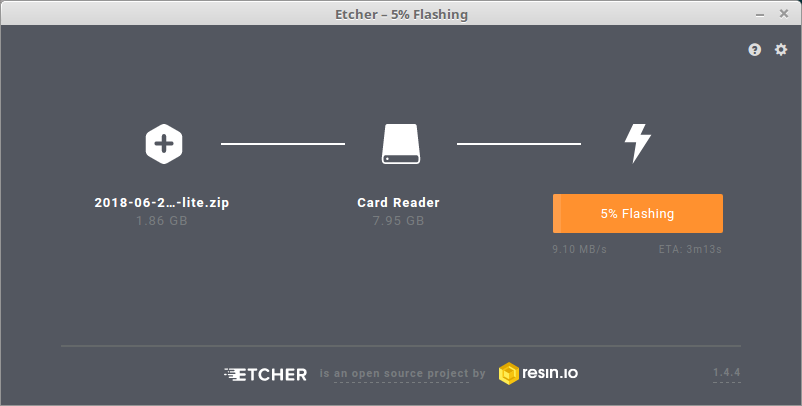
\includegraphics[width=0.5\linewidth]{figures/Etcher_flashing.png}
	\caption{Etcher flashing image to microSD card}
	\label{fig:etcher_flashing}
\end{figure}

If everything went as expected, the \gls{Rpi} will start to boot and prepare the first setup. It will be seen led light blinking indicating activity. After a few minutes, it should be possible to access it remotely via ssh

%-------------------------------------------------------------------------------
% create a remote access setup
%-------------------------------------------------------------------------------

\subsection{Remote access}
The next step is to find the ip address of the \gls{Rpi}. For example, in linux terminal type \console{arp -a}. In figure \ref{arp_example} is seen an output example. In red stroke is shown the \gls{MAC} address of a \gls{Rpi}. Every \gls{MAC} is unique and the first three bytes are fixed in every \gls{Rpi} wich correspond to organizationally unique identifier \cite{mac_wiki} associated to Raspberry Pi Foundation, B8:27:EB \cite{wireshark_mac}.

\begin{figure}[hb]
	\centering
	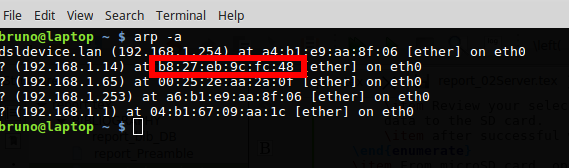
\includegraphics[width=0.7\textwidth]{figures/arp_example}
	\caption{arp -a command example output}
	\label{arp_example}
\end{figure}

Perform the first login with using the default login details as shown in table \ref{tab:default_login}.
Using the discovered ip for the \gls{Rpi}, in Linux, the first login  may be performed using \console{ssh pi@\textless ip-of-Rpi\textgreater} command and entering the default password.
\begin{table}[h]
	\centering
	\begin{tabular}{rl}
		\toprule
		\textbf{username:}& pi\\
		\textbf{password:}& raspberry\\
		\bottomrule
	\end{tabular}
	\caption{Default login details for \gls{Rpi}}
	\label{tab:default_login}
\end{table}

\begin{figure}[hb]
	\centering
	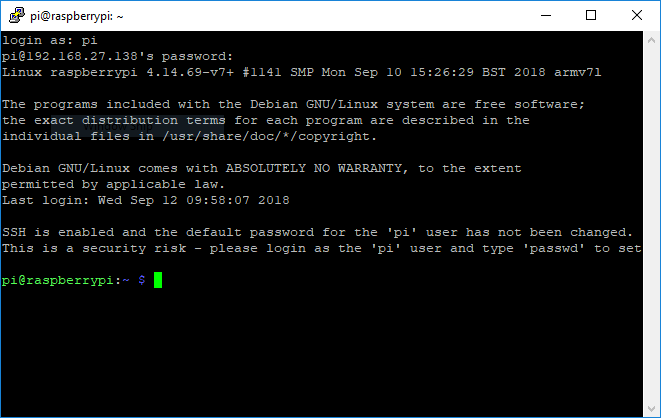
\includegraphics[width=0.7\textwidth]{figures/ssh_sucessfull.png}
	\caption{SSH sucessfull login}
	\label{fig:ssh_successfull}
\end{figure}

%-------------------------------------------------------------------------------
%  initial update and configurations 
%-------------------------------------------------------------------------------
\subsection{Initial update and configuration}
If the user as been granted with permission to login, the next steps are used to perform a few tweaks.
To do that user must use the command \console{sudo raspi-config}. Example output is seen in figure \ref{fig:raspi_config}.

\begin{figure}[hb]
	\centering
	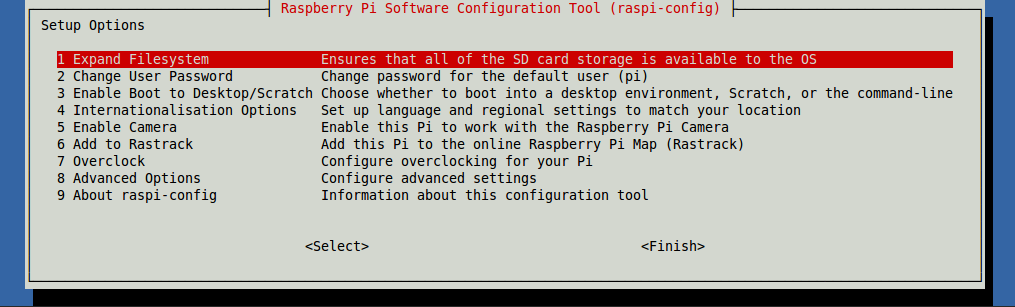
\includegraphics[width=0.7\textwidth]{figures/raspi-config}
	\caption{Raspi-config example output}
	\label{fig:raspi_config}
\end{figure}

\begin{itemize}
	\tightlist
	\item Set Keyboard Layout
	\item Update to lastest software
	\item Set Timezone
	\item Set language [optional]
	\item Change default login password
	\item Configure Wifi-zone [if present]
	\item Enable \gls{SPI} for \gls{CAN} controller
	\item Enable \gls{I2C} for RTC
	\item Set hostname
	\item change default password
	\item change memory for GPU
\end{itemize}



The current settings are presented in table \ref{tab:suggested_config}. 

\begin{table}[h]
	\centering
	\begin{tabular}{rl}
		\toprule
		\textbf{Username:}& pi\\
		\textbf{Password:}& fiatelettra\\
		\textbf{Hostname:}& raspberrypi\\
		\textbf{wait for network at boot:}& no\\
		\textbf{Language:}& en\_GB.UTF-8 UTF-8\\
	    \textbf{Timezone:}& Europe $\rightarrow$ Lisbon\\
	    \textbf{Keyboard layout:}& pt\_PT\\
	    \textbf{WIFI country:}& PT\_Portugal\\
	    \textbf{SPI:}& on\\	
		\textbf{I2C:}& on\\
		\textbf{Memory split:}& 16 (minimum since is running headless)\\
		\bottomrule
	\end{tabular}
	\caption{Suggested details for \gls{Rpi}}
	\label{tab:suggested_config}
\end{table}

After successfully changed the settings, perform a full update and upgrade by running:
\begin{lstlisting}[frame=none,language=bash,backgroundcolor=\color{gray!15},numbers=none]
sudo apt update && sudo apt upgrade -y
\end{lstlisting}


\section{Prepare CAN interface}
\label{section:can}
The current protoboard uses the \gls{IC} \href{https://www.microchip.com/wwwproducts/en/MCP2515}{MCP2515} as \gls{CAN} network controller and \href{https://www.microchip.com/wwwproducts/en/MCP2551}{MCP2551} as \gls{CAN} transceiver. Figure \ref{fig:proto_can} shows the used protoboard with highlighted connections names and parts.

The schematic circuit implemented in the protoboard is present in figure \ref{fig:schematic_proto_can}.
Current raspbian kernel, automatically support the can interaction via \gls{SPI} to \gls{IC} MCP2515, making it available via SocketCAN. To enable that, it is necessaries to configure MCP2515 driver on device tree overlay and install the can-utils package.
\begin{itemize}
	\tightlist
	\item Install can-utils using \console{sudo apt install can-utils}
	\item Enable MCP2515 overlay by using \console{sudo nano /boot/config.txt} and append at end:
	\begin{lstlisting}[label={lst:boot_settings},frame=none,language=bash,backgroundcolor=\color{gray!15},numbers=none,basicstyle=\ttfamily]
		#CAN bus controllers
		dtoverlay=mcp2515-can0,oscillator=16000000,interrupt=25
		dtoverlay=spi-bcm2835
\end{lstlisting}
	\item To enable the interface at boot time, use \console{sudo nano /etc/network/interfaces} and append at end:
	\begin{minipage}{\linewidth} % to avoid breaking on page
\begin{lstlisting}[frame=none,language=bash,backgroundcolor=\color{gray!15},numbers=none,		basicstyle=\ttfamily]
		auto can0
		iface can0 inet manual
		  pre-up /sbin/ip link set can0 type can bitrate 1000000 \ 
		  triple-sampling on restart-ms 10
		  up /sbin/ifconfig can0 up
		  down /sbin/ifconfig can0 down
\end{lstlisting}
	\end{minipage}
\end{itemize}
This will enable the \gls{CAN} interface at boot time with the setting present in table \ref{tab:can_settings}.


\begin{figure}[hb]
	\begin{minipage}{0.49\linewidth}
		\centering
		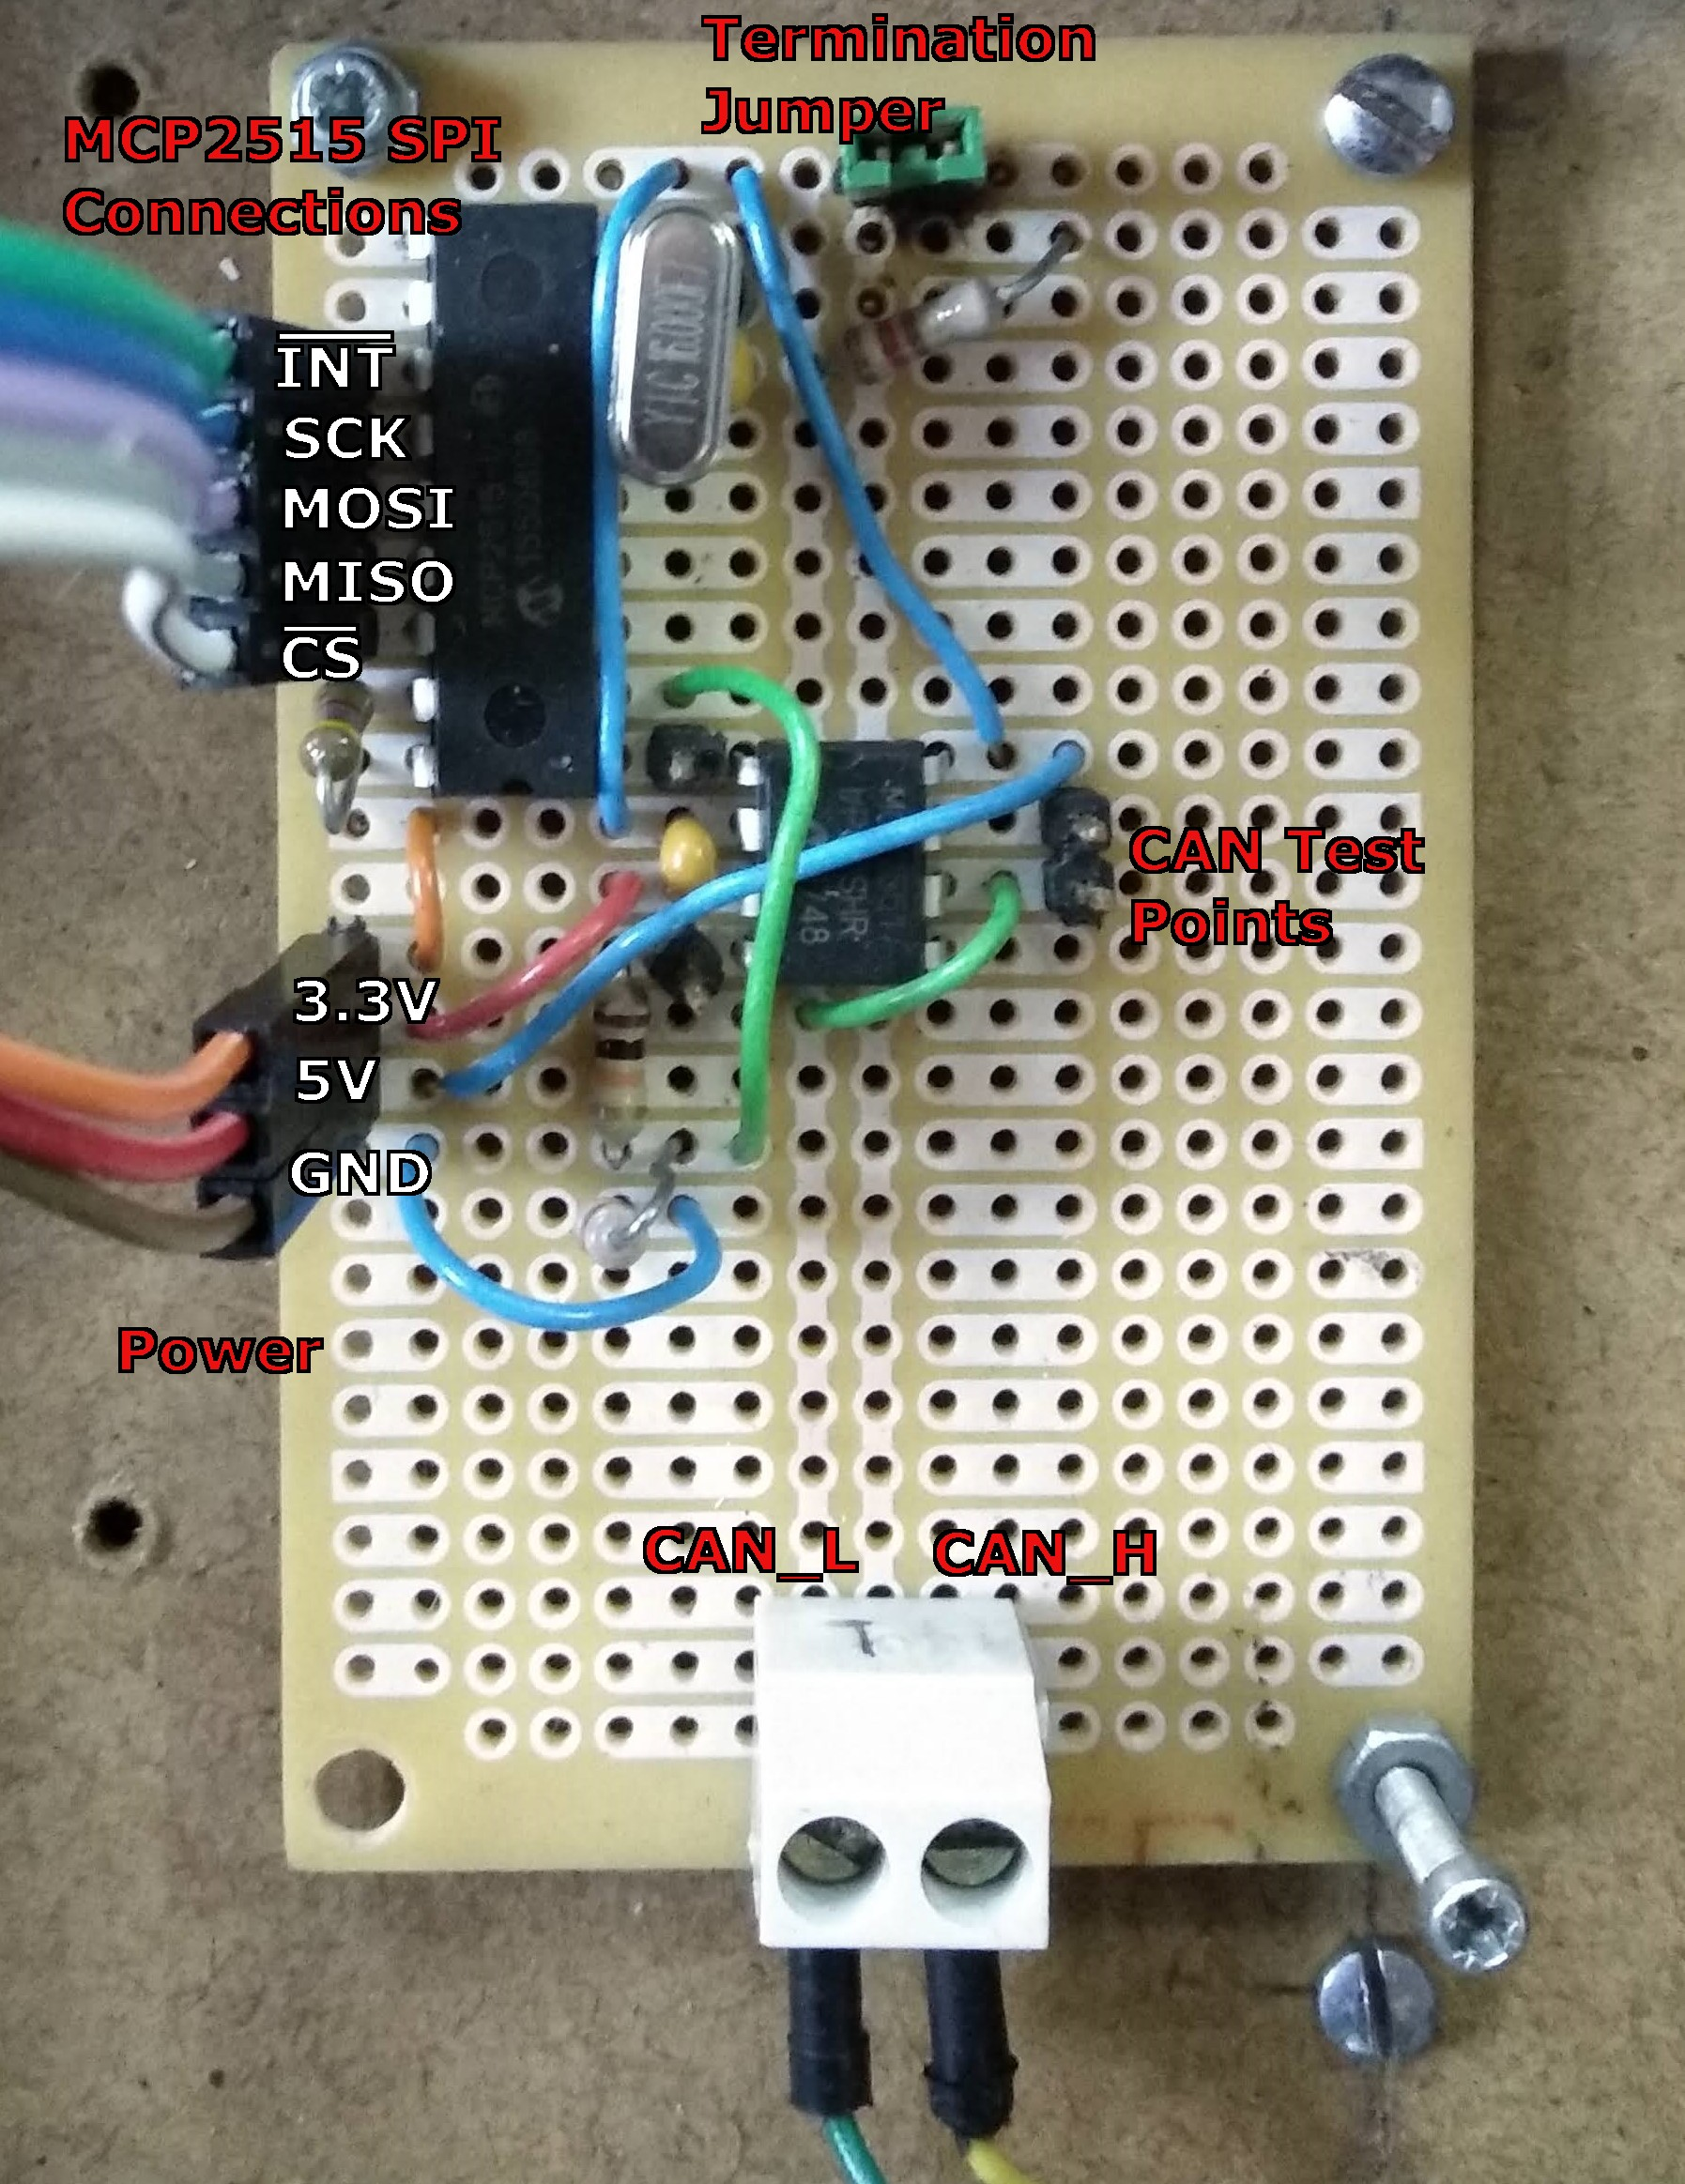
\includegraphics[width=1\linewidth]{figures/proto_can}
		\caption{Protoboard designed for CAN interface}
		\label{fig:proto_can}
	\end{minipage}
	\begin{minipage}{0.49\linewidth}
		\centering
		\begin{tabular}{rl}
			\toprule
			\textbf{Parameter} & \textbf{Value}\\
			\midrule
			Bitrate & 1Mbps\\
			Triple Sampling & on\\
			Sampling point & 0.75\\
			Restart & 10ms\\
			\bottomrule
		\end{tabular}
	    \captionof{table}{CAN used settings}
	    \label{tab:can_settings}
	\end{minipage}
\end{figure}

\begin{figure}[!hb]
	\centering
	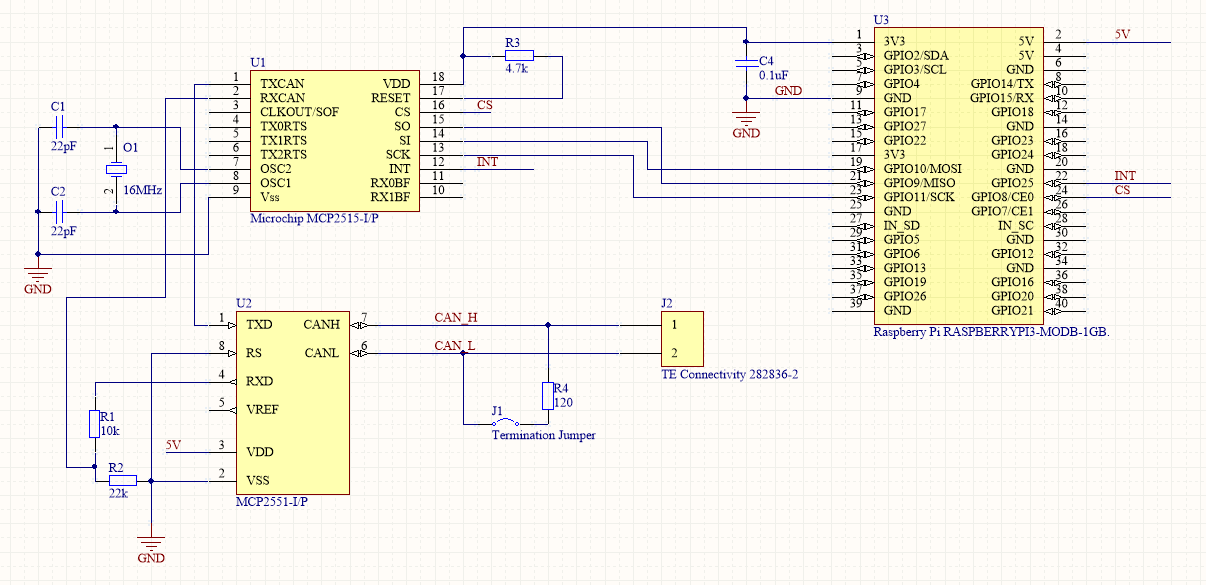
\includegraphics[width=0.9\linewidth]{figures/protoschematic}
	\caption{CAN protoboard schematic}
	\label{fig:schematic_proto_can}
\end{figure}



%-------------------------------------------------------------------------------
% create a additional packages installation
%-------------------------------------------------------------------------------
\section{Additional packages installation}
The following list describes additional package installation that are currently used or are planned to be used.
\begin{description}[style=nextline]
	\item[python3-pip] Required to enable pip manager.
	\item[python3-venv] To enable the creation of virtual environments.
	\item[libatlas-base-dev] Required to install numpy package.
	\item[mosquitto] Local \gls{MQTT} broker used currently in development branch. It might be useful to install also the \console{mosquitto-clients}.
	\item[build-essential] Required if need to compile anything.
	\item[git] Add git support to raspbian.
	\item[nginx] Local lightweight web server application used to control or see current status of vehicle (in development) 
	\item[ufw] Firewall interface to improve security.
	\item[dnsmasq] Provides network infrastructure for small networks as \gls{DNS}, \gls{DHCP}. Will be used to configure \gls{Rpi} as an \gls{AP}.
	\item[hostapd] Daemon for configuring and enabling the \gls{AP}
\end{description}

\section{Post-Installation Procedures}
After installing the recommend packages, user should perform several configurations. In this section is described each of them.

\subsection{Adding user to groups}
After adding user to any group, \textbf{a logout must be performed to changes take effect}. Changes can be confirmed by using the command \console{groups} that prints the groups current user is in.
\begin{description}[style=nextline]
	\item[www-data] Grant user ability to perform changes on /var/www. Run \console{sudo adduser pi www-data}
	\item[dialout] Grant user ablility to use ports. Run \console{sudo adduser pi dialout}
\end{description}

%-------------------------------------------------------------------------------
% installing mosquitto
%-------------------------------------------------------------------------------
\subsection{Configuring MQTT Broker}
Current and planned development roadmap use MQTT brocker to change messages between user or high level software and hardware interface. It is also used websockets and in this section will be shown how to enable it. The currently  broker is \href{https://mosquitto.org/}{mosquitto}. If not already installed, use:\\ \console{sudo apt install mosquitto} \\
After installation edit mosquitto.conf by using \console{sudo nano /etc/mosquitto/mosquitto.conf} and add an additional port for websockets protocol. If advanced configuration is need refer to \cite{mosquitto_conf}.
\begin{lstlisting}[frame=none,language=bash,backgroundcolor=\color{gray!15},numbers=none,		basicstyle=\ttfamily]
pid_file /var/run/mosquitto.pid
persistence true
persistence_location /var/lib/mosquitto/

log_dest file /var/log/mosquitto/mosquitto.log

include_dir /etc/mosquitto/conf.d

port 1883
listener 8080
protocol websockets
\end{lstlisting}

\subsection{Configuring Rpi as AP}
While in development user is advised to use ehternet connection between developement PC and \gls{Rpi}, it is useful to configure \gls{Rpi} as an \gls{AP} so users can connect to it using wifi in field environment. Here will be assumed that internet connection is provided via ethernet cable during development phase, for example via host PC, and during normal operation \gls{Rpi} will not be connected to internet. This section follows the main instructions given in \cite{raspberry_AP}.
\begin{itemize}
	\tightlist
	\item Turn off hostapd and dnsmasq. Perform this using systemctl with:
	\begin{lstlisting}[frame=none,language=bash,backgroundcolor=\color{gray!15},numbers=none,		basicstyle=\ttfamily]
sudo systemctl stop dnsmasq
sudo systemctl stop hostapd
\end{lstlisting}
	\item Configuring a static IP. Edit \console{/etc/dhcpcd.conf} with nano and change the file as shown below, assuming the user wants to assign the server IP address as 192.168.4.1, using wlan0 as interface.
	\begin{lstlisting}[frame=none,language=bash,backgroundcolor=\color{gray!15},numbers=none,		basicstyle=\ttfamily]
# static ip address for wlan0 to be used as AP
interface wlan0
    static ip_address=192.168.4.1/24
    nohook wpa_supplicant
\end{lstlisting}
   	\item Restart dhcpd using \console{sudo service dhcpcd restart}
   	\item Configuring the DHCP server (dnsmasq). Perform a copy of original file and create a new one
\begin{lstlisting}[frame=none,language=bash,backgroundcolor=\color{gray!15},numbers=none,		basicstyle=\ttfamily]
sudo mv /etc/dnsmasq.conf /etc/dnsmasq.conf.orig  
sudo nano /etc/dnsmasq.conf
\end{lstlisting}
   	On new opened configuration file place that will allow dhcp on interface wlan0 giving ip addresses to clients from 192.168.4.2 to 192.168.4.20 with a lease time of 24h:
   	\begin{lstlisting}[frame=none,language=bash,backgroundcolor=\color{gray!15},numbers=none,		basicstyle=\ttfamily]
interface=wlan0
dhcp-range=192.168.4.2,192.168.4.20,255.255.255.0,24h
\end{lstlisting}
   	\item Configuring the access point host software (hostapd). Table \ref{tab:ap_settings} show the suggested SSID and password. Edit file /etc/hostapd/hostapd.conf and add:
\begin{lstlisting}[frame=none,language=bash,backgroundcolor=\color{gray!15},numbers=none,		basicstyle=\ttfamily]
interface=wlan0
driver=nl80211
ssid=VIENA
hw_mode=g
channel=7
wmm_enabled=0
macaddr_acl=0
auth_algs=1
ignore_broadcast_ssid=0
wpa=2
wpa_passphrase=fiatelettra
wpa_key_mgmt=WPA-PSK
wpa_pairwise=TKIP
rsn_pairwise=CCMP
\end{lstlisting}
Now edit file \console{sudo nano /etc/default/hostapd} and add to it:\\ \console{DAEMON\_CONF="/etc/hostapd/hostapd.conf"}
\item Restart services: 
\begin{lstlisting}[frame=none,language=bash,backgroundcolor=\color{gray!15},numbers=none,		basicstyle=\ttfamily]
sudo systemctl start hostapd
sudo systemctl start dnsmasq
\end{lstlisting}
\item Edit /etc/sysctl.conf and uncomment line \console{net.ipv4.ip\_forward=1}
\item Add a masquerade for outbound traffic on ehternet port:
\begin{lstlisting}[frame=none,language=bash,backgroundcolor=\color{gray!15},numbers=none,		basicstyle=\ttfamily]
sudo iptables -t nat -A  POSTROUTING -o eth0 -j MASQUERADE
sudo sh -c "iptables-save > /etc/iptables.ipv4.nat"
\end{lstlisting}
\item Edit /etc/rc.local and add this just above \console{exit 0} to install these rules on boot:
\begin{lstlisting}[frame=none,language=bash,backgroundcolor=\color{gray!15},numbers=none,		basicstyle=\ttfamily]
iptables-restore < /etc/iptables.ipv4.nat
\end{lstlisting}
\item Reboot. After it user should be able to connect to configured network and current user authentication settings.
\end{itemize}

\begin{table}[hb]
	\centering
	\begin{tabular}{rl}
		\toprule
		\textbf{SSID} & VIENA\\
		\textbf{password} & fiatelettra\\
		\bottomrule
	\end{tabular}
    \caption{Suggested AP login settings}
    \label{tab:ap_settings}
\end{table}

\subsection{Configure Nginx}
\blindtext

\subsection{Configure firewall}
First enable firewall by using \console{sudo ufw enable}. After use the following console command to enable the previously configured ports for ssh connection, mqtt connections and http server configured in nginx:
\begin{lstlisting}[frame=none,language=bash,backgroundcolor=\color{gray!15},numbers=none,		basicstyle=\ttfamily]
sudo ufw allow 22
sudo ufw allow 80
sudo ufw allow 1883
sudo ufw allow 8080
sudo ufw allow 80
\end{lstlisting}
If needed, confirm status with \console{sudo ufw status}. For more advanced use run \console{man ufw}.

%-------------------------------------------------------------------------------
% create a Troubleshooting section
%-------------------------------------------------------------------------------
\section{Troubleshooting}

\begin{description}[style=nextline]
	\item [The command \console{arp -a} do not show my \gls{Rpi}] In that case, try use the \console{sudo nmap -sS 192.168.1.0/24}, assuming the 192.168.1.0/24 is your local network. This is a time consuming command!
    %---------------------------------------------------------------------------	
	\item [Cannot find my \gls{Rpi} IP. Is it even running?] Maybe there is some problem with boot or bad microSD reading. The easiest solution is to connect a monitor and keyboard. Check messages at boot time. If nothing seems strange, manually login and then check if ehternet connection is ok using \console{ifconfig}
	%---------------------------------------------------------------------------
	\item [\gls{CAN} seems to not be working] First see if MCP2515 is successfully connected. 
	\begin{enumerate}
		\item Use \console{dmesg \textbar grep mcp2515*}. If it says successfull configured, go to next step. If not, recheck connections and restart. Also make sure the oscilator frequency match the used on boot configuration file settings as seen \hyperref[lst:boot_settings]{\textcolor{cyan}{here}}.
		\item Check if can is detected as a socketcan interface. Use \console{ifconfig}. If \gls{CAN} is available, it should show a section for can0. If not, re-check if can-utils is installed.
		\item View details about \gls{CAN} connection. use \console{ip -details -statistics link show can0} to get more information. If current state is \console{BUS-OFF}, manually restart the \gls{CAN} by using the following:
		\begin{lstlisting}[frame=none,language=bash,backgroundcolor=\color{gray!15},numbers=none,		basicstyle=\ttfamily]
		sudo ip link set can0 down
		sudo ip link set can0 up \end{lstlisting}
	\end{enumerate}
\end{description}
 % file "Thesis_Background.tex"
\clearpage

\chapter{Code Guidelines}
In this chapter is described the main guidelines used for coding and documentation as well as relevant suggestions.
Since the majority of code is developed in Python, the guidelines are provided for that language. However similar suggestion may apply for the other languages cases. Here follows a list of sugestions:
\begin{description}
	%-----------------------------------------------------------------------
	% Git
	%-----------------------------------------------------------------------
	\item [Git] \hfill \\The first suggestion is the code version control system, Git. It has a lot integrations with majority of IDE's and have lot of free tools to manage it. It allows easy contributions from multiple users. Documentation and guides to become familiar with it can be found at \href{https://try.github.io/}{try.github.io}
	\item[Python3] \hfill \\ Since Python core team is dropping support for python 2.7.x in 2020 \cite{python_end_of_life} and some of important package developers are also dropping support for it \cite{numpy_end_of_life}, the chosen \textbf{version is the 3.X.}
	%-----------------------------------------------------------------------
	% Virtual environment
	%-----------------------------------------------------------------------
	\item[Use virtual environment] \hfill\\ Typically, every Linux distribution uses python to run critical routines. Perturbing the main ecosystem of python packages should be avoided, at least during development phase. Raspbian is no exception, so it is suggested to use virtual environments. It is used to create a isolated local installation in the directory you are working. Since version 3.5 the official recommended tool for creating virtual environments is the venv \cite{python_doc}.
	To create a virtual environment use the following console command \console{python3 -m venv /path/to/new/virtual/environment} or  assuming the user is currently in desired local path, simplify to \console{python3 -m venv .} 
	To activate/deactivate the local environment follow the specification accordingly to used \gls{OS} as present in table \ref{tab:venv_activate}, using the same assumption as before. After activation, the shell prefix will change from the default to \console{(\textless path of venv\textgreater)} which is a easy away to check if environment is active or not.
	
	\begin{table}[hb]
		\centering
		\begin{tabular}{lll}
			\toprule
			\multicolumn{1}{c}{\textbf{Shell}} & \multicolumn{1}{c}{\textbf{Activate}} & \multicolumn{1}{c}{\textbf{Deactivate}}\\
			\midrule
			\multicolumn{3}{c}{POSIX}\\
			\midrule
			bash/zsh & source ./bin/activate & deactivate\\
			fish & source ./bin/activate.fish & deactivate\\
			csh/tcsh & source ./bin/activate.csh & deactivate\\
			\midrule
			\multicolumn{3}{c}{Windows}\\
			\midrule
			cmd & .\textbackslash Scripts\textbackslash activate.bat & deactivate\\
			PowerShell & .\textbackslash Scripts\textbackslash Activate.ps1 & deactivate\\
			\bottomrule
		\end{tabular}
		\caption{Activation/deactivation of venv OS specific}
		\label{tab:venv_activate}
	\end{table}
	%-----------------------------------------------------------------------
    % Requirements
    %-----------------------------------------------------------------------
	\item[Requirements files (requirements.txt)] \hfill \\Requirement files are an easy away to install all the requisites necessary to run the code and ensure repeatability of installations. Unless any particular reason, a restriction of any package version should be avoided. Requirements file can be as simple as a list of necessary packages or more complex struture, if needed \cite{python_requirements}. Installation of requirements is done by running the following command \console{pip install -r requirements.txt}
	%-----------------------------------------------------------------------
	% Google style guide
	%-----------------------------------------------------------------------
	\item[Google style docstrings] \hfill \\ A good documentation is a key point for keeping good readability of a project. Docstrings format from Google Style Guide \cite{python_google_style} is adopted. Many projects can fail from bad documentation.
	%-----------------------------------------------------------------------
	% Sphinx and napolean
	%-----------------------------------------------------------------------
	\item[Sphinx with automation] \hfill \\ Similar to previous point, \href{http://www.sphinx-doc.org/en/master/}{sphinx} will allow the auto documentation generation from code. Is a popular tool for creating documentation and is used also in \href{https://readthedocs.org}{readthedocs.org}, that allows to integrate documentation update with commits in the three main git repository management services, GitHub, Bitbucket, and GitLab. Using autodoc and napoleon extension allow an easy maintenance of code documentation.
	%-----------------------------------------------------------------------
	% Argparse
	%-----------------------------------------------------------------------
	\item[Argparse] \hfill \\ Use \href{https://docs.python.org/3/library/argparse.html}{argparse} to create clean and readable argument handling if necessary. It auto generates help, description and handles unknown options.
	%-----------------------------------------------------------------------
	% logging module
	%-----------------------------------------------------------------------
	\item[Logging] \hfill \\ Since the main intention is to run programs in a headless computer, the \href{https://docs.python.org/3/library/logging.html}{logging module} should be used instead of typical print() function. Not only it helps keep tracking of events defined in code, but also keeps track of other modules events. It also allows the creation of multiple destinations using the handlers and each handler can have its own format. Typical handlers used in project are files, console and websockets (currently only in development branchs)
\end{description}




 





\clearpage

\chapter{Batteries}
\blindtext

\section{Main battery packs}
\blindtext

\section{Auxiliary battery pack}
\blindtext

\clearpage


\chapter{NovatelOEM4 GPS Library}\label{welcome-to-novateloem4-gps-librarys-documentation}

\begin{description}
\item[Date]
24 Jul 2018
\item[Version]
0.4
\item[Author]
Bruno Tibério
\item[Contact]
\href{mailto:bruno.tiberio@tecnico.ulisboa.pt}{\nolinkurl{bruno.tiberio@tecnico.ulisboa.pt}}
\end{description}

This module contains a few functions to interact with Novatel OEM4 GPS
devices. Currently only the most important functions and definitions are
configured, but the intention is to make it as much complete as
possible.

A simple example can be run by executing the main function wich creates
a Gps class object and execute the following commands on gps receiver:

\begin{itemize}
\tightlist
\item
  \textbf{begin:} on default port or given port by argv{[}1{]}.
\item
  \textbf{sendUnlogall}
\item
  \textbf{setCom(baud=115200):} changes baudrate to 115200bps
\item
  \textbf{askLog(trigger=2,period=0.1):} ask for log \emph{bestxyz} with
  trigger {ONTIME} and period {0.1}
\item
  wait for 10 seconds
\item
  \textbf{shutdown:} safely disconnects from gps receiver
\end{itemize}

\begin{lstlisting}[language=python,frame=none,backgroundcolor=\color{gray!15},numbers=none]
$python NovatelOEM4.py
\end{lstlisting}


\section{Changelog}
\label{\detokenize{index:changelog}}\begin{quote}\begin{description}
		\item[{version 0.4}] \leavevmode
		Moved from optoparse to argparse module.
		changed Queue to make it compatible with python3 queue. Backwards compatibility is maintained.
		Restructured default location. Moved from Lib folder to base path.
		Moved examples to proper folder. This cause backwards compatibility problems. On import, replace
		\console{import Lib.NovatelOEM4} with simply \console{import NovatelOEM4}
		
		\item[{version 0.3}] \leavevmode
		logging configuration as moved outside module to enable user to use already
		configured logging handler. Check \href{https://docs.python.org/2/howto/logging-cookbook.html\#using-logging-in-multiple-modules{}`}{multimodule logging docs}
		
\end{description}\end{quote}
\begin{quote}\begin{description}
		\item[{version 0.2}] \leavevmode
		data from bestxyz message is now placed into a Queue.Queue() FIFO
		
		\item[{version 0.1}] \leavevmode
		initial release
\end{description}\end{quote}

\section[class NovatelOEM4.Gps]{\prefix{class NovatelOEM4.}\textbf{Gps}\args{sensorName='GPS'}}
Novatel OEM4 GPS library class

This class contents is an approach to create a library for Novatel OEM 4 GPS
\begin{quote}
\begin{description}[style=nextline]
		\item[Parameters] \leavevmode
		\sphinxbfcode{sensorName} (optional) \textendash{} A sensor name if used with multiple devices.
		\item[Returns] An object of class NovatelOEM4.Gps	
\end{description}
\end{quote}

\subsection{askLog}
\noindent \prefix{Gps.}\textbf{askLog}\args{logID=’BESTXYZ’, port=192, trigger=4, period=0, offset=0, hold=0}
Request a log from receiver.
\begin{quote}\begin{description}
		\item[{Parameters}] \leavevmode
		\begin{itemize}
			\item \textbf{logID} \textendash{} log type to request.
			
			\item \textbf{port} \textendash{} port to report log.
			
			\item {} 
			\sphinxstyleliteralstrong{trigger} \textendash{} trigger identifier.
			
			\item \textbf{period} \textendash{} the period of log.
			
			\item \textbf{offset} \textendash{} offset in seconds after period.
			
			\item \textbf{hold} \textendash{} mark log with hold flag or not.
			
		\end{itemize}
		
		\item[{Returns}] \leavevmode
		True or false if command was sucessfull or not.
		
\end{description}\end{quote}

The log request command is defined as:





\clearpage

% ----------------------------------------------------------------------
%  Bibliography
% ----------------------------------------------------------------------

% Add entry in the table of contents as chapter
\phantomsection
\addcontentsline{toc}{chapter}{\bibname}

% Include all references in .bib file, even non-cited ones...
%\nocite{*} % this should be used carefully because it is not correct!

% Produces the bibliography section when processed by BibTeX
%
% Bibliography style
% > entries ordered alphabetically
%\bibliographystyle{plain}
% > unsorted with entries appearing in the order in which the citations appear.
%\bibliographystyle{unsrt}
% > entries ordered alphabetically, with first names and names of journals and 
%months abbreviated
%\bibliographystyle{abbrv}
% > entries ordered alphabetically, with reference markers based on authors' 
%initials and publication year
%\bibliographystyle{alpha}
%
% Replacement bibliography styles provided by 'natbib' package
% (plainnat.bst, abbrvnat.bst, unsrtnat.bst )
% > entries ordered alphabetically
%\bibliographystyle{plainnat}
% > unsorted with entries appearing in the order in which the citations appear.
%\bibliographystyle{unsrtnat}
% > entries ordered alphabetically, with first names and names of journals and 
%months abbreviated
%\bibliographystyle{abbrvnat} % <<<<< SELECT IF USING REFERENCES BY AUTHOR/YEAR
% > entries ordered alphabetically, with reference markers based on authors' 
%initials and publication year
%\bibliographystyle{alpha}
%
% Custom bibliography style adapted from 'natbib' package
%   (based on 
%http://tex.stackexchange.com/questions/5053/is-it-possible-to-get-unsrt-abbrv-bibliography)
%   (unsrtnat.bst + abbrvnat.bst -> abbrvunsrtnat.bst)
%   (original files copied from:
%   http://tug.ctan.org/macros/latex/contrib/natbib/abbrvnat.bst
%   http://tug.ctan.org/macros/latex/contrib/natbib/unsrtnat.bst
% > unsorted with entries appearing in the order in which the citations appear, 
%with first names and names of journals and months abbreviated.
\bibliographystyle{abbrvunsrtnat} % <<<<< SELECT IF USING REFERENCES BY NUMBER 
%(CITATION ORDER)

% External bibliography database file in the BibTeX format
\bibliography{report_bib_DB} % file "Thesis_bib_DB.bib"
\clearpage

% ----------------------------------------------------------------------
%  Appendix (optional)
%
%  CAUTION: 1) the main document (up to the conclusions) shall not exceed 80 
%pages
%           2) the document shall not exceed a total of 100 pages (per IST 
%regulations)
% ----------------------------------------------------------------------
%\appendix
%
%% add page number prefix according to apendix chapter (optional)
%%\renewcommand{\thepage}{\thechapter.\arabic{page}}
%
%% re-set arabic numbering (A.1,A.2,...) (optional, use only if chapter prefix 
%%is added)
%%\setcounter{page}{1}
%
%\input{Thesis_Appendix_A} % file "Thesis_Appendix_A.tex"
%\cleardoublepage


% ----------------------------------------------------------------------
\end{document}
% ----------------------------------------------------------------------
